\documentclass[11pt,nocut]{article}

\usepackage{../latex_style/packages}
\usepackage{../latex_style/notations}
%\externaldocument{../lecture_02/lecture_02}
\externaldocument{../lecture_07/lecture_07}


\title{\vspace{-2.0cm}%
	Optimization and Computational Linear Algebra for Data Science\\
Lecture 10: Optimality conditions}
\author{Léo \textsc{Miolane} \ $\cdot$ \ \texttt{leo.miolane@gmail.com}}
\date{\today}

\begin{document}
\maketitle
\textbf{Warning:}
\emph{This material is not meant to be lecture notes. It only gathers the main concepts and results from the lecture, without any additional explanation, motivation, examples, figures...
}


\section{Local and global minimizers}

We aim at minimizing a function $f: \R^n \to \R$.
We say that $x^* \in \R^n$ is
\begin{itemize}
	\item a \emph{global} minimizer of $f$ if for all $x \in \R^n$, $f(x^*) \leq f(x)$.
	\item a \emph{local} minimizer of $f$ if there exists $\delta > 0$ such that for all $x \in B(x^*,\delta)$, $f(x^*) \leq f(x)$.
\end{itemize}
Of course, a global minimizer if also a local minimizer but the converse is not true.

\begin{proposition}\label{prop:zero_grad}
	Let $x \in \R^n$ be a point at which $f$ is differentiable. 
	Then
	$$
	x \ \text{is a local minimizer of} \ f \ \implies \nabla f(x) = 0.
	$$
\end{proposition}

If $f$ is convex then the converse is true:

\begin{proposition}\label{prop:zero_grad_convex}
	Assume that $f$ is convex.
	Let $x \in \R^n$ be a point at which $f$ is differentiable. 
	Then
	$$
	\nabla f(x) = 0 \ \implies \ x \ \text{is a global minimizer of} \ f.
	$$
\end{proposition}

\section{Constrained optimization}

We would now like to investigate constrained optimization problems:
\begin{equation}\label{eq:problem}
\begin{array}{lll}
	\text{minimize} & f(x) & \\
	\text{subject to} & g_i(x) \leq 0, & i=1, \dots, m \\
					  & h_i(x) = 0, & i=1, \dots, p,
\end{array}
\end{equation}
with variable $x \in \R^n$.
Here we have $m$ inequality constraints $g_1(x) \leq 0, \dots, g_m(x)\leq  0$ and $p$ equality constraints $h_1(x) = 0, \dots, h_p(x) = 0$ to satisfy.

\begin{definition}[Feasible point]
	A point $x \in \R^n$ is \emph{feasible} if it satisfies all the constraints: $g_1(x) \leq 0, \dots, g_m(x)\leq  0$ and $h_1(x) = 0, \dots, h_p(x) = 0$. We will denote by $F$ the set of feasible points.
\end{definition}

We would now get for the problem \eqref{eq:problem} the analog of Proposition \ref{prop:zero_grad}.
Since an equality constraint $h_i(x) = 0$ can be equivalently written in two inequality constraints $h_i(x) \leq 0$ and $-h_i(x) \leq 0$, we can assume to have only inequality constraints.
For simplicity, we first assume to have only one inequality constraint $g(x) \leq 0$ so that \eqref{eq:problem} reduces to
\begin{equation}\label{eq:problem2}
\text{minimize} \ f(x) \ \text{subject to} \ g(x) \leq 0.
\end{equation}


Let $x$ be a solution of \eqref{eq:problem2}, i.e.\ $g(x) \leq 0$ and $f(x) \leq f(x')$ for all $x'$ such that $g(x')\leq0$
We distinguish two cases:

\paragraph{Case 1: $x$ is ``strictly feasible'' $g(x) <0$.} In that case $x$ is in the interior of $F$: one can find $\delta > 0$ such that $B(x,\delta) \subset F$. Since $x$ is a solution of \eqref{eq:problem2} we have for all $x' \in B(0,\delta)$, $f(x) \leq f(x')$. One can therefore apply Proposition \ref{prop:zero_grad} to get that $\nabla f(x) = 0$.

We conclude that in the case where the constraint is not active, the constraint does not play any role and one gets the same optimality condition as in the unconstrained setting.

\paragraph{Case 2: the constraint is active in $x$, $g(x) = 0$.}
In that case, there exists $\lambda \geq 0$ such that 
\begin{equation}\label{eq:grad_active}
\nabla f(x) = - \lambda \nabla g(x).
\end{equation}
To see that, assume that \eqref{eq:grad_active} does not hold. Then we are in the following situation:
\begin{figure}[h!]
	\begin{center}
	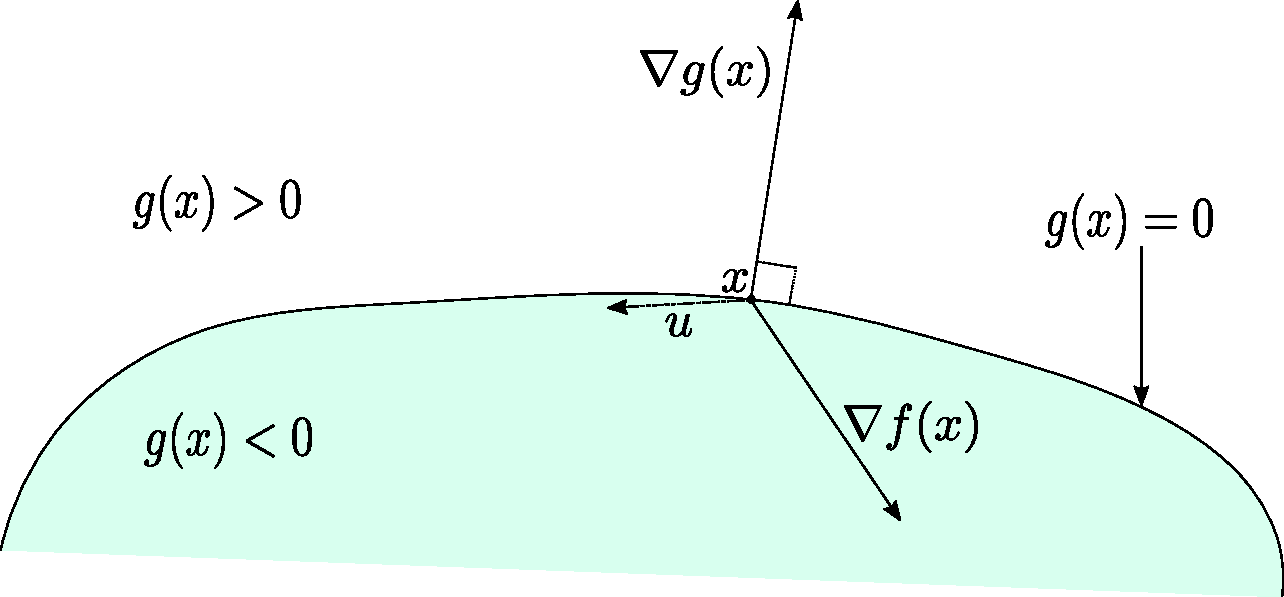
\includegraphics[width=0.8\linewidth]{figures/absurd.pdf}
	\end{center}
\end{figure}

As we can see on the figure, we can find a vector $u$ such that
$$
\langle u, \nabla g(x) \rangle < 0 
\quad \text{and} \quad
\langle u, \nabla f(x) \rangle < 0.
$$
Starting from $x$ and following the direction $u$ one remains in the feasible set because for small $\delta >0$
$$
g(x + \delta u) \simeq g(x) + \delta \langle u, \nabla g(x) \rangle \leq 0.
$$
Moreover, $f$ decreases locally on the direction $u$:
$$
f(x + \delta u) \simeq f(x) + \delta \langle u, \nabla f(x) \rangle < f(x).
$$
This means that one can find $\delta > 0$ such that $x + \delta u$ is feasible and such that $f(x + \delta u) < f(x)$. This contradicts the assumption that $x$ is solution of \eqref{eq:problem2}.
We conclude that \eqref{eq:grad_active} holds, i.e.\ that there exists $\lambda \geq 0$ such that
$$
\nabla f(x) + \lambda \nabla g(x) = 0.
$$

We will only cover the case where the equality constraints are linear, i.e. $h_i(x) = \langle a_i, x \rangle + b_i$ for from $a_i \in \R^n$ and $b_i \in \R$.

This generalize to the case \eqref{eq:problem} where we have multiple constraints:

\begin{definition}
	We say that the constraints are \emph{qualified} at $x \in F$ if there exists a vector $v \in \R^n$ such that
	\begin{itemize}
		\item $\langle v, \nabla g_i \rangle < 0$ for all $i=1,\dots, m$.
		\item $\langle v, \nabla h_i \rangle = 0$ for all $i=1, \dots, p$.
	\end{itemize}
\end{definition}

\begin{theorem}[Karush-Kuhn-Tucker conditions]
	Assume that the functions $f$, $g_1, \dots, g_m$ are differentiable and that $h_1, \dots, h_p$ are linear. If $x$ is solution of \eqref{eq:problem} and if the constraints are qualified at $x$
	then there exists $\lambda_1, \dots, \lambda_m \geq 0$ and $\nu_1, \dots, \nu_p \in \R$ such that:
	\begin{equation}\label{eq:kkt}
	\nabla f(x) + \sum_{i=1}^m \lambda_i \nabla g_i(x) + \sum_{i=1}^p \nu_i \nabla h_i(x) = 0.
\end{equation}
	Moreover $\lambda_i = 0$ if $g_i(x) < 0$.
\end{theorem}

The scalars $\lambda_i, \nu_i$ are often called \emph{Lagrange multipliers}.

\section{The Lagrange dual function}

We define the Lagrange dual function $L$ associated with the problem \eqref{eq:problem} by
\begin{equation}
	L(x,\lambda,\nu) = 
	f(x) + \sum_{i=1}^m \lambda_i g_i(x) + \sum_{i=1}^p \nu_i h_i(x),
\end{equation}
where $x \in \R^n$, $\lambda \in \R_{\geq 0}^m$ and $\nu \in \R^p$. We define the Lagrange dual function by
$$
\ell(\lambda,\nu) = \inf_{x \in \R^n} L(x,\lambda,\nu).
$$
Notice that for all feasible point $x$,
$$
L(x,\lambda,\nu)
= f(x) + \sum_{i=1}^m \lambda_i g_i(x) \leq f(x)
$$
because $h_i(x) = 0$ and $\lambda_i g_i(x) \leq 0$. By taking the infimum in $x$ on both sides of the inequality we get a lower bound on the value of the optimization problem \eqref{eq:problem}:
\begin{proposition}
	For all $\lambda_1, \dots, \lambda_m \geq 0$ and all $\nu_1, \dots,\nu_p \in \R$ we have:
	\begin{equation}\label{eq:dual_lower_bound}
\ell(\lambda,\nu) \leq \inf_{x \in \R^n} f(x).
	\end{equation}
\end{proposition}

We would like to make the lower bound \eqref{eq:dual_lower_bound} as tight as possible: one would like therefore to solve the so-called \emph{dual problem}:
\begin{equation}\label{eq:dual_problem}
\begin{array}{lll}
	\text{maximize} & \ell(\lambda,\nu) & \\
	\text{subject to} & \lambda_i \geq 0, & i=1, \dots, m \\
					  & \nu_i \in \R, & i=1, \dots, p.
\end{array}
\end{equation}

From \eqref{eq:dual_lower_bound} we deduce that the optimal value of the primal problem is greater or equal than the one of the dual problem:
\begin{equation}
	\sup_{\lambda \geq 0, \nu} \ell(\lambda,\nu) \leq \inf_{x \in \R^n} f(x).
\end{equation}
This is known as \emph{weak duality}.
\\

Notice that the original optimization problem \eqref{eq:problem} can be rewritten as
$$
\text{minimize} \quad \sup_{\lambda \geq 0, \nu} L(x,\lambda,\nu) \quad \text{in the variable} \quad x \in \R^n.
$$
Indeed,
$$
\sup_{\lambda \geq 0, \nu} L(x,\lambda,\nu)
=
\begin{cases}
	f(x) & \text{if} \ x \ \text{is feasible},\\
	+ \infty & \text{otherwise.}
\end{cases}
$$
Hence, the weak duality inequality can be rewritten as:
\begin{equation}
	\sup_{\lambda \geq 0, \nu} \inf_{x \in \R^n} L(x,\lambda,\nu) \leq \inf_{x \in \R^n} \sup_{\lambda \geq 0, \nu} L(x,\lambda,\nu).
\end{equation}

\section*{Further reading}

See \cite{von2007tutorial} for a very nice introduction to spectral clustering and \cite{spielman2012spectral} for lecture notes on spectral graph theory.

\vspace{1cm}
\centerline{\pgfornament[width=7cm]{71}}


\bibliographystyle{plain}
\bibliography{../references.bib}
\end{document}
